\documentclass{beamer}

\usetheme{Madrid}
\usecolortheme{beaver}
\graphicspath{{./figures/}}

\makeatother
\setbeamertemplate{footline}
{
  \leavevmode%
  \hbox{%
  \begin{beamercolorbox}[wd=.2\paperwidth,ht=2.25ex,dp=1ex,center]{author in head/foot}%
    \usebeamerfont{author in head/foot}\insertshortauthor
  \end{beamercolorbox}%
  \begin{beamercolorbox}[wd=.8\paperwidth,ht=2.25ex,dp=1ex,center]{title in head/foot}%
    \usebeamerfont{title in head/foot}\insertshorttitle\hspace*{3em}
    \insertframenumber{} / \inserttotalframenumber\hspace*{1ex}
  \end{beamercolorbox}}%
  \vskip0pt%
}
\makeatletter
\setbeamertemplate{navigation symbols}{}

\AtBeginSection[]{
  \begin{frame}
  \vfill
  \centering
  \begin{beamercolorbox}[sep=8pt,center,shadow=true,rounded=true]{title}
    \usebeamerfont{title}\insertsectionhead\par%
  \end{beamercolorbox}
  \vfill
  \end{frame}
}

\title{Technology comparison for interface selection in mmWave Vehicular Networks}
\author{Davide Peron}
\date{\today}


\begin{document}

	\maketitle

	\begin{frame}{Outline}
		\tableofcontents
	\end{frame}


	\section{Introduction}

	\begin{frame}{Introduction}
		In the near future, vehicles will communicate each other for several reasons. Nowadays technologies are not suitable for every kind of application. \vspace{.5em}

		A set of technologies have to cohexist to ensure good connection in every situation \vspace{.5em}
	\end{frame}

	\begin{frame}{Introduction}
		In this work a comparison between the following three technologies is made: \vspace{.5em}
		\begin{itemize}
			\item IEEE 802.11p / DSRC\vspace{.5em}
			\item LTE \vspace{.5em}
			\item mmWaves
		\end{itemize}
	\end{frame}


	\section{DSRC}

	\begin{frame}{DSRC Introduction}
		\begin{itemize}
			\item Used for a V2V scenario
			\item \textbf{Physical data rate: } $6Mb/s$\vspace{.5em}
			\item \textbf{Bandwidth: } 10MHz\vspace{.5em}
			\item \textbf{Application data rates simulated: } $10kb/s$, $100Mb/s$, $1Gb/s$
			\item \textbf{Packet Size: } 1000 bytes
		\end{itemize}
	\end{frame}

	\begin{frame}{DSRC Simulation Scenario}
		\begin{itemize}
			\item 2 vehicles in Line-of-Sight share data using UDP\vspace{.5em}
			\item Distance increases from 2 meters to 200 meters\vspace{.5em}
			\item 15 runs for each distance and for each data rate
		\end{itemize}
	\end{frame}

	\begin{frame}{DSRC Results}
		\begin{columns}
			\column{0.5\textwidth}
				\begin{figure}
					\vspace{-0.1in}
					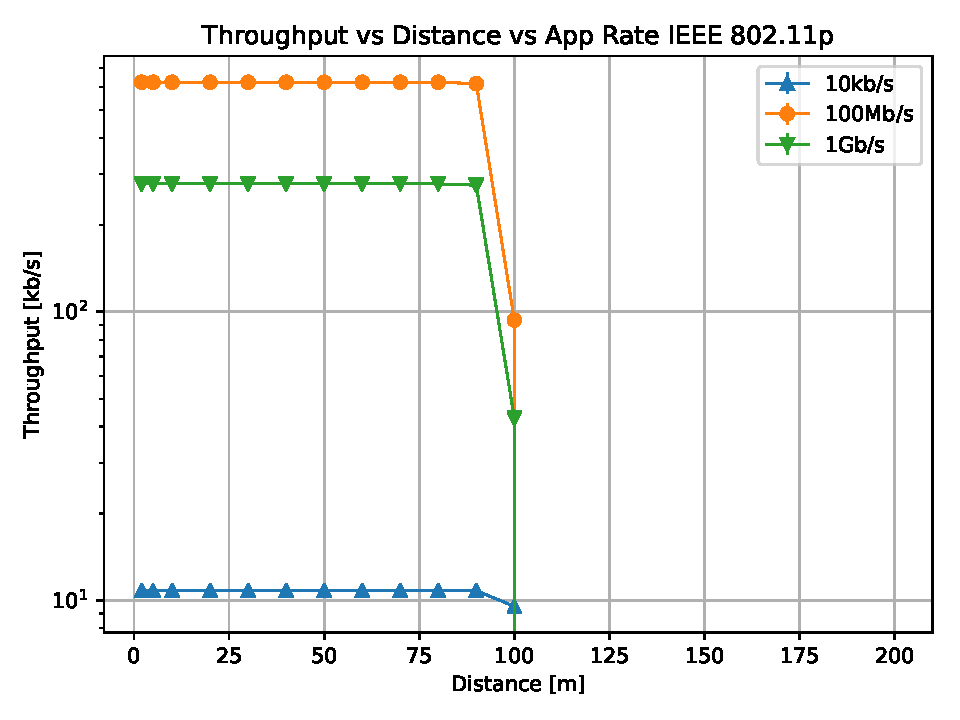
\includegraphics[scale=0.28]{throughput_distance_wave_UDP}
				\end{figure}
				\begin{figure}
					\vspace{-0.2in}
					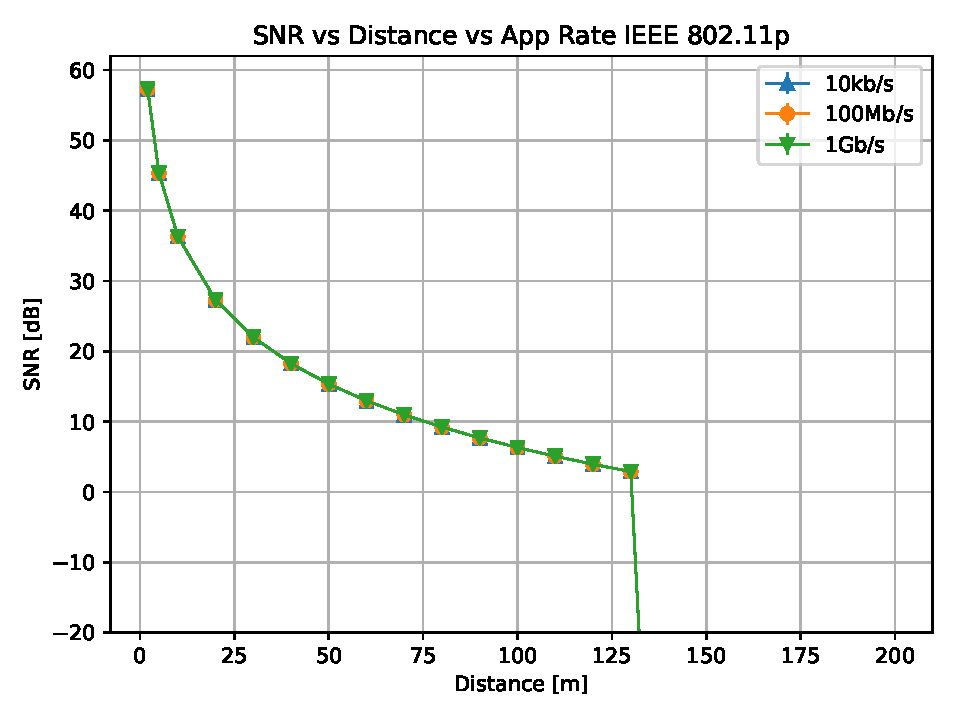
\includegraphics[scale=0.28]{SNR_distance_wave_UDP}
				\end{figure}
			\column{0.5\textwidth}
				\begin{figure}
					\vspace{-0.1in}
					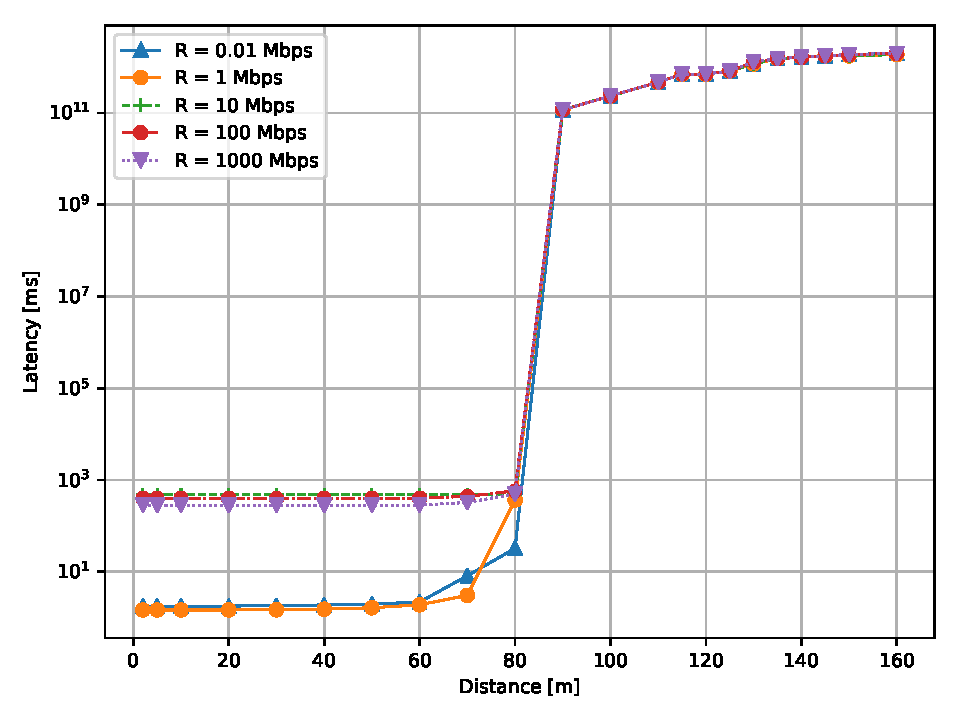
\includegraphics[scale=0.28]{latency_distance_wave_UDP}
				\end{figure}
				\begin{figure}
					\vspace{-0.2in}
					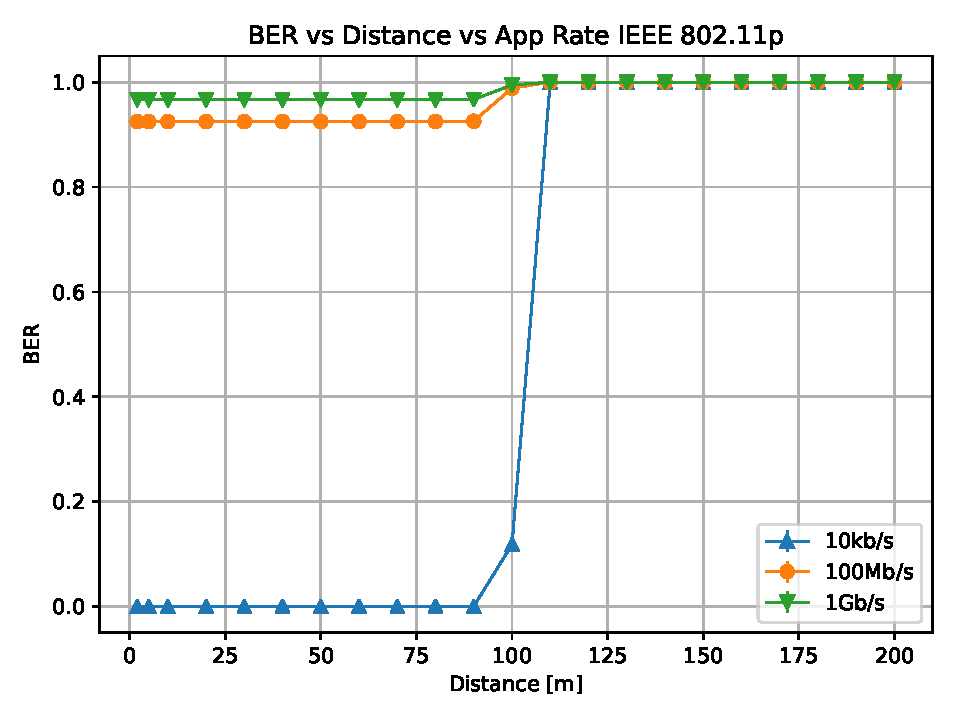
\includegraphics[scale=0.28]{BER_distance_wave_UDP}
				\end{figure}
		\end{columns}
	\end{frame}

	\section{LTE and mmWaves}

	\begin{frame}{Simulated scenario}
		These technologies have been simulated for a V2I scenario, in a square area 500 meters wide with 6 buildings and an increasing number of base stations randomly positioned.\vspace{.5em}
		The number of base stations increases from 3 to 40, the User Equipment moves $30m/s$ and sends packets of 1000 bytes each.
		\begin{figure}
			\vspace{-0.1in}
			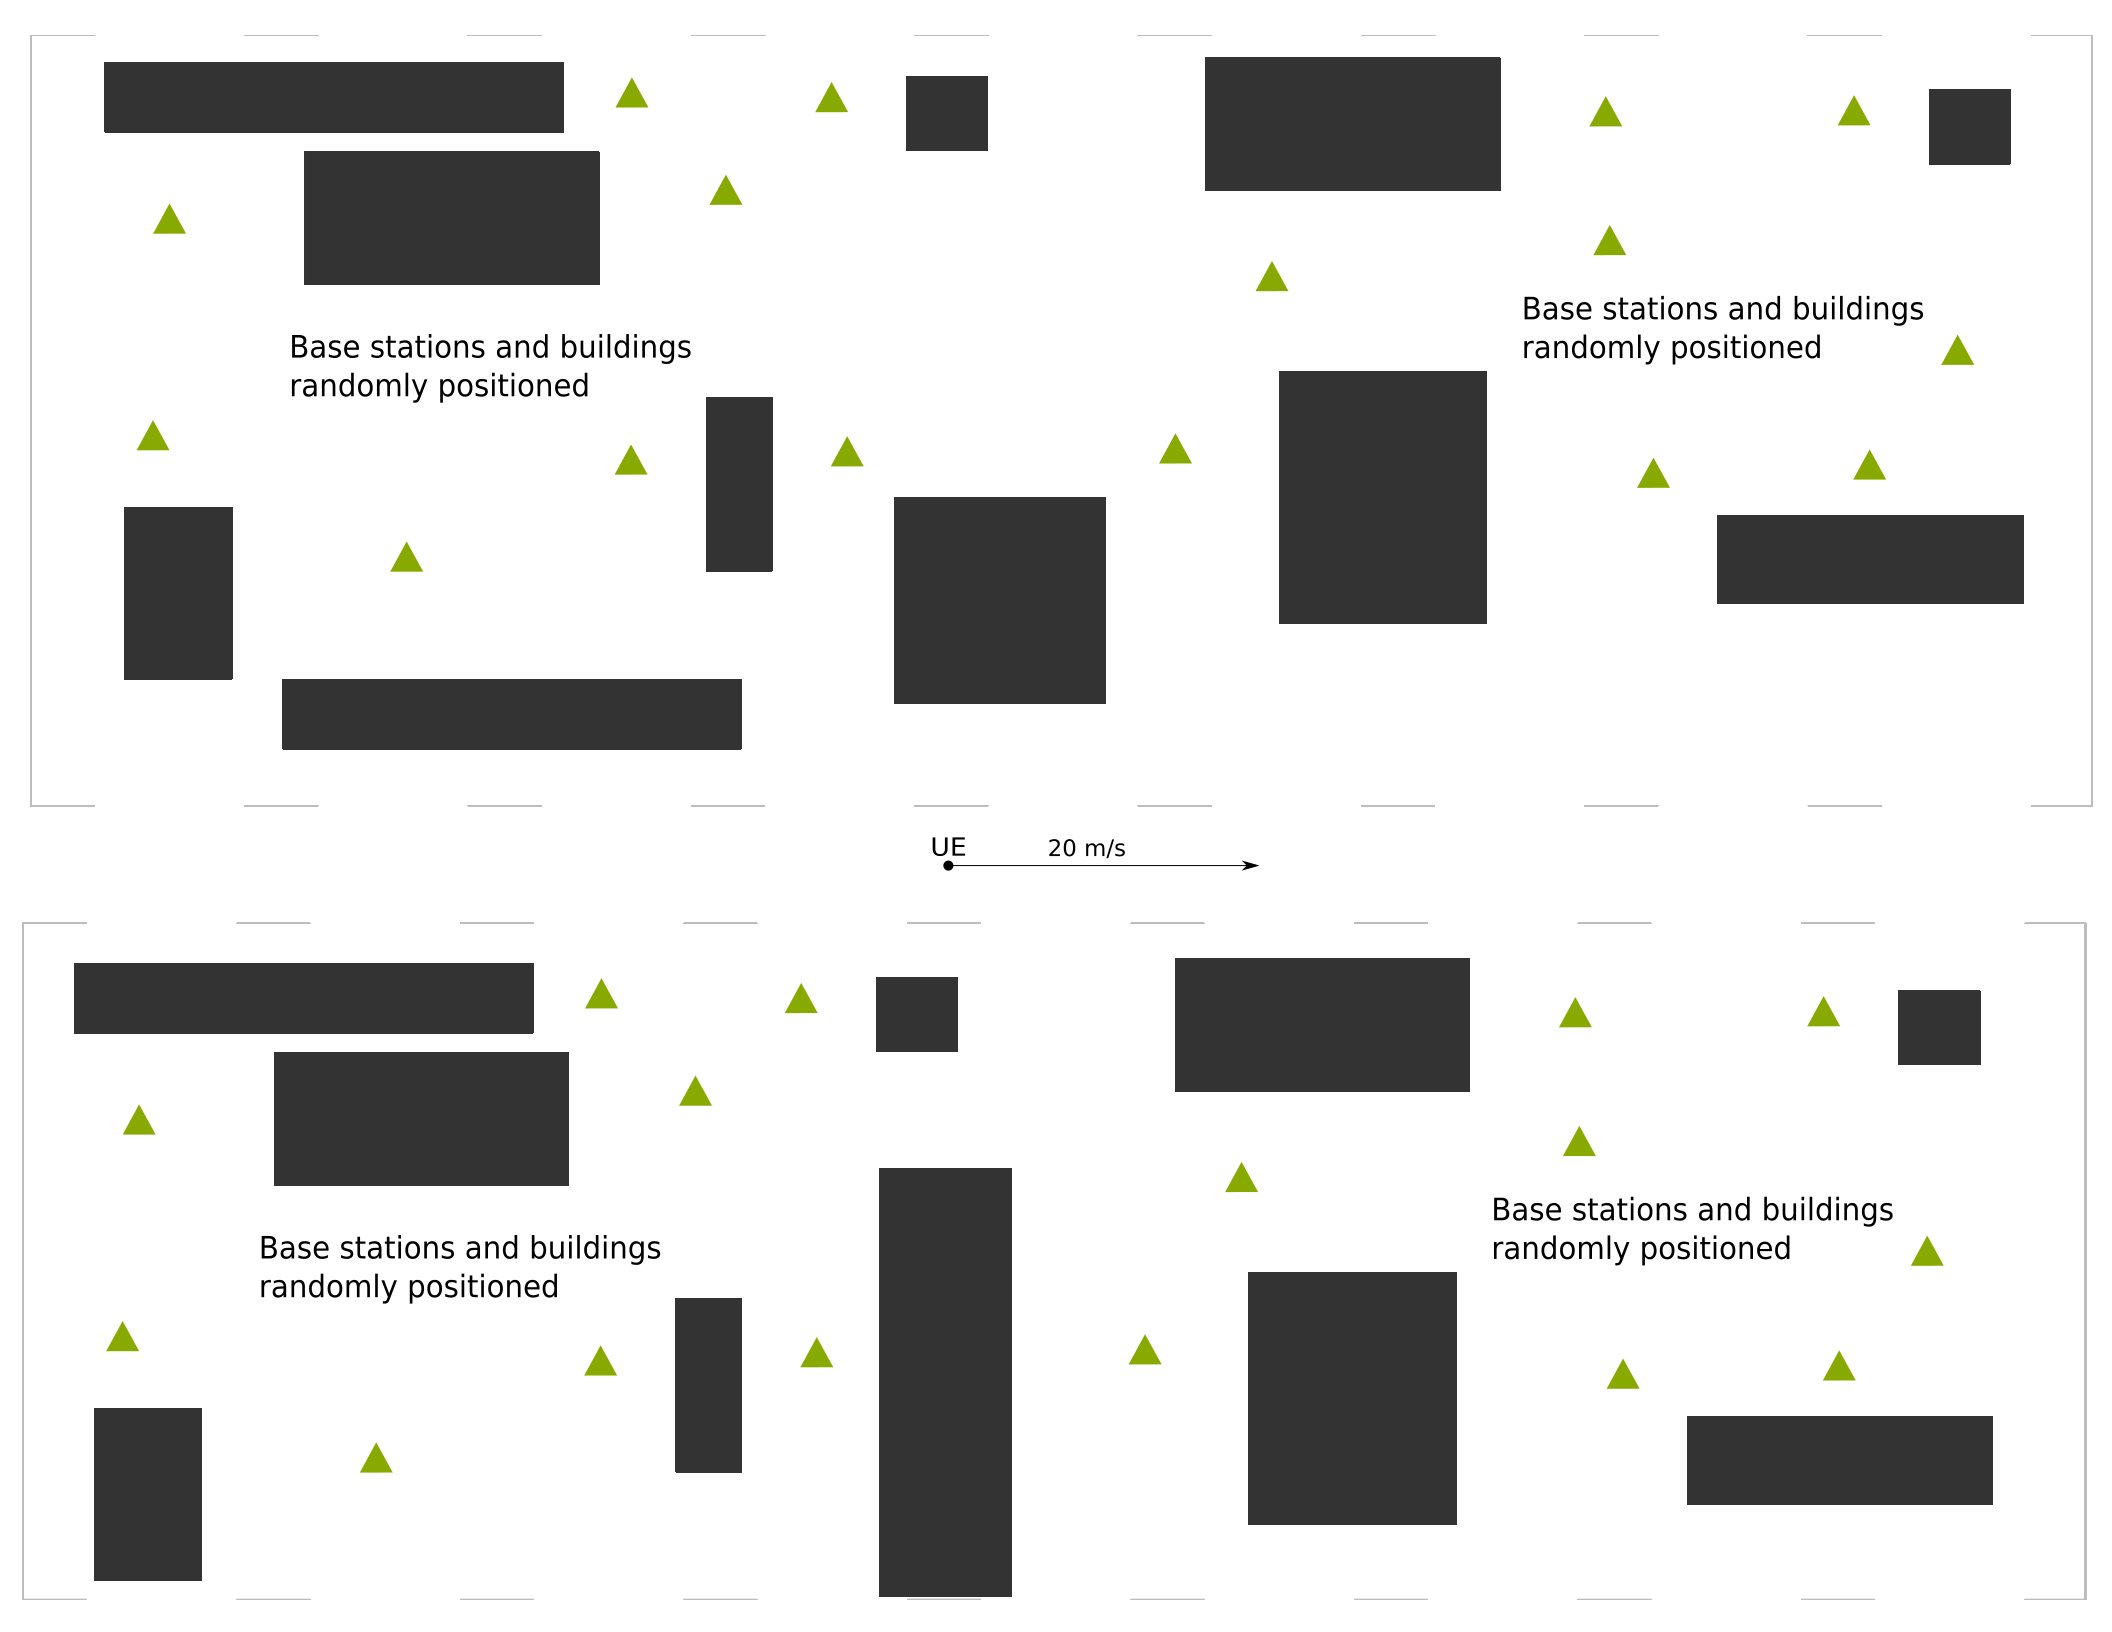
\includegraphics[scale=0.18]{scenario}
		\end{figure}
	\end{frame}

	\begin{frame}{LTE and mmWaves results}
		\begin{columns}
			\column{0.5\textwidth}
				\begin{figure}
					\vspace{-0.1in}
					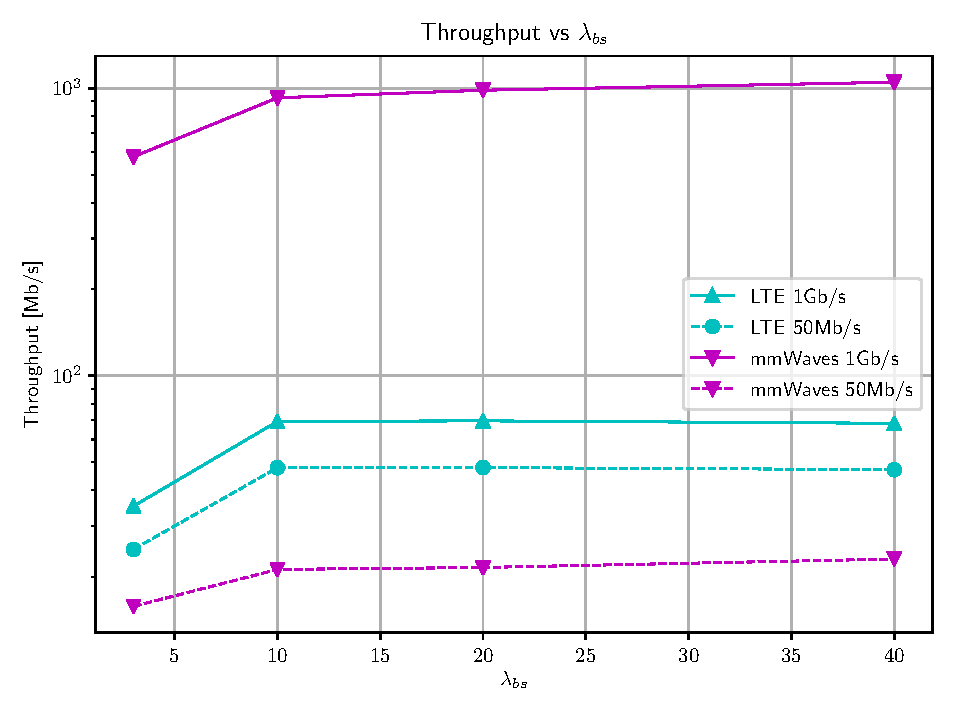
\includegraphics[scale=0.28]{throughput_lambda_bs_lte_mmwave_UDP}
				\end{figure}
				\begin{figure}
					\vspace{-0.2in}
					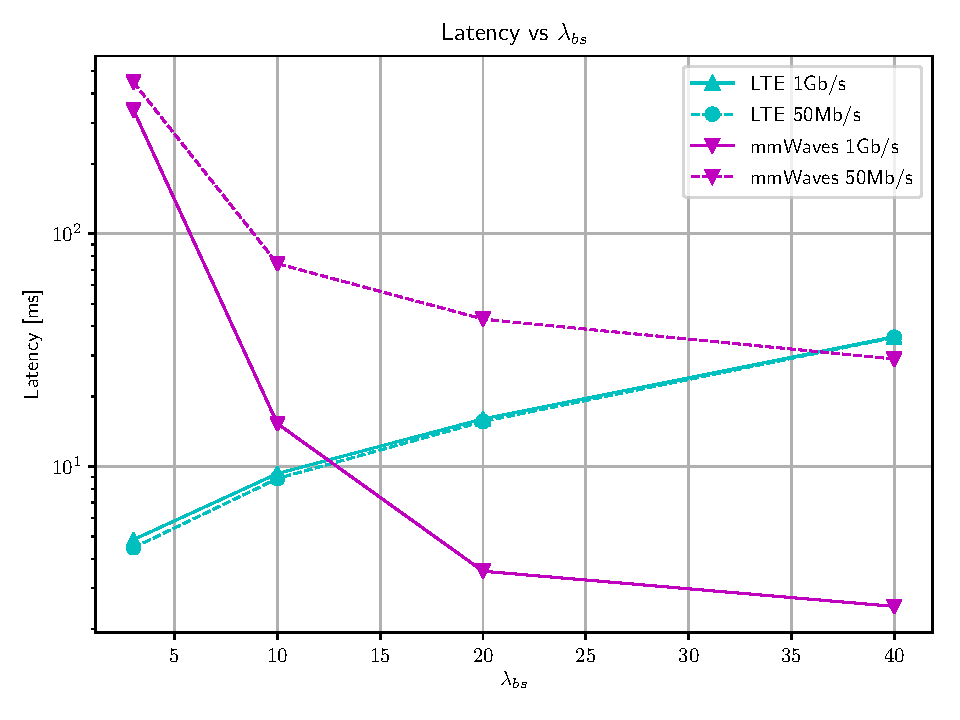
\includegraphics[scale=0.28]{latency_lambda_bs_lte_mmwave_UDP}
				\end{figure}
			\column{0.5\textwidth}
				\begin{figure}
					\vspace{-0.1in}
					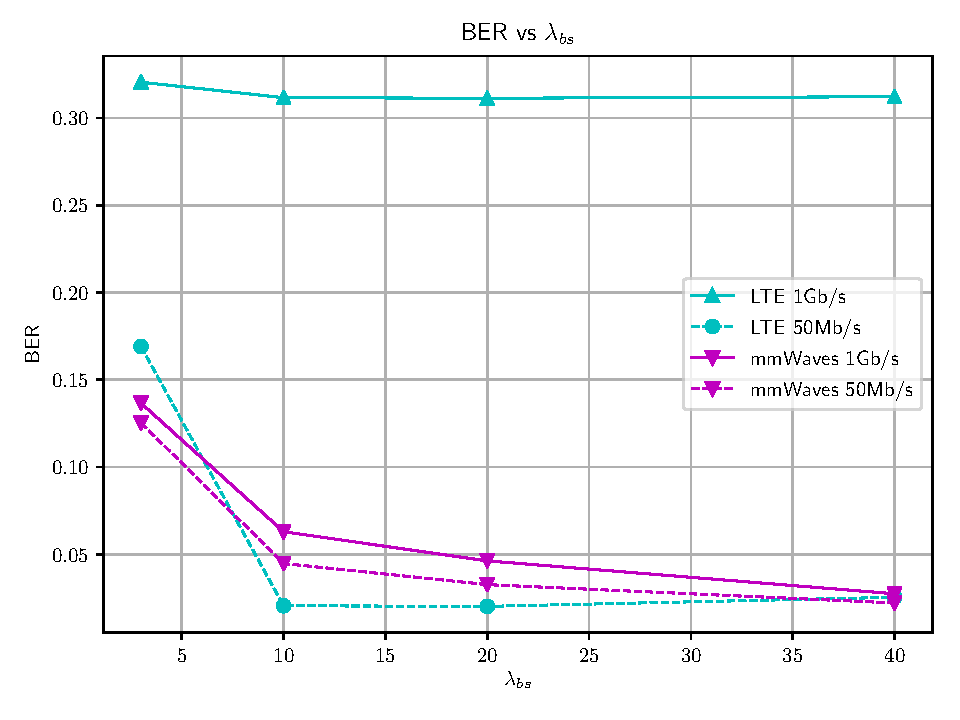
\includegraphics[scale=0.28]{BER_lambda_bs_lte_mmwave_UDP}
				\end{figure}
				\begin{figure}
					\vspace{-0.2in}
					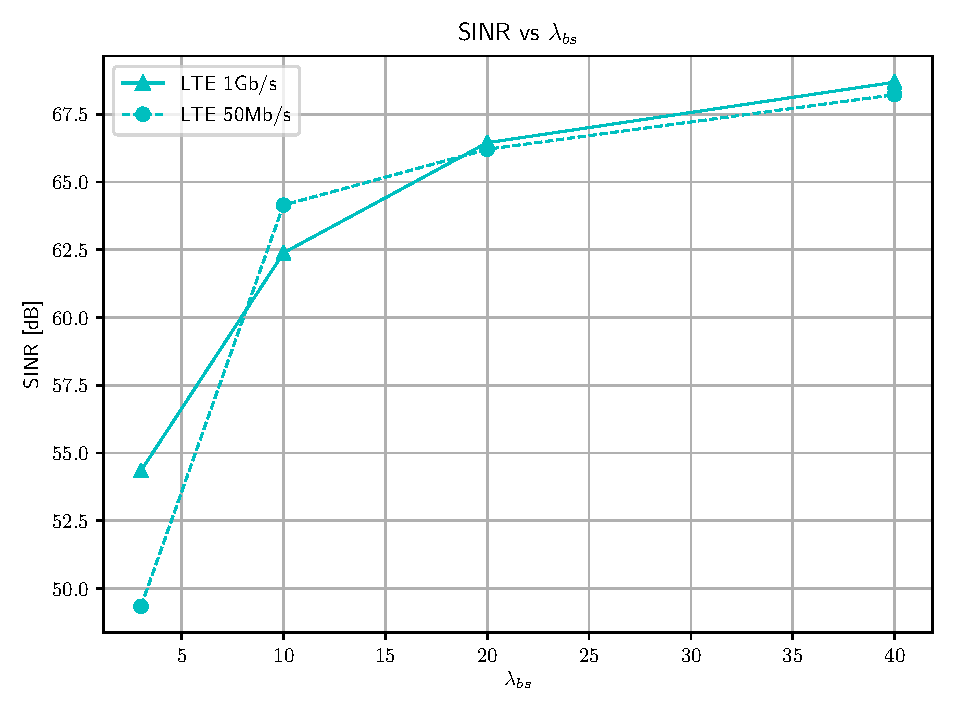
\includegraphics[scale=0.28]{SINR_lambda_bs_lte_mmwave_UDP}
				\end{figure}
		\end{columns}
	\end{frame}

	\begin{frame}{LTE and mmWaves single run}
		\begin{columns}
			\column{0.5\textwidth}
				\begin{figure}
					\vspace{-0.1in}
					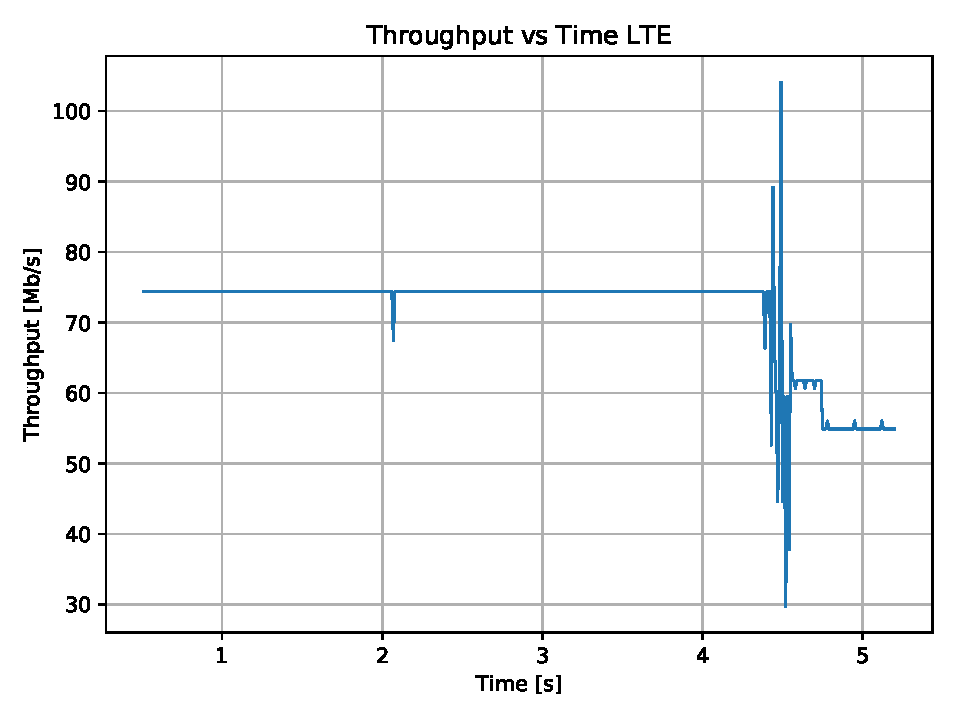
\includegraphics[scale=0.28]{throughput_lte_UDP}
				\end{figure}
				\begin{figure}
					\vspace{-0.2in}
					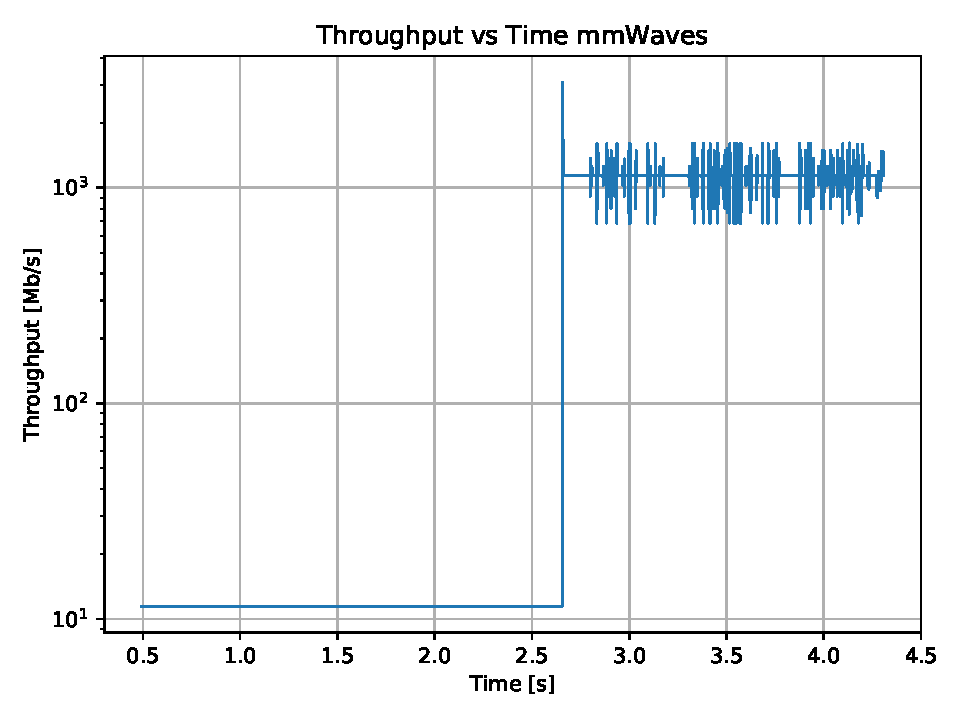
\includegraphics[scale=0.28]{throughput_mmWaves_UDP}
				\end{figure}
			\column{0.5\textwidth}
				\begin{figure}
					\vspace{-0.1in}
					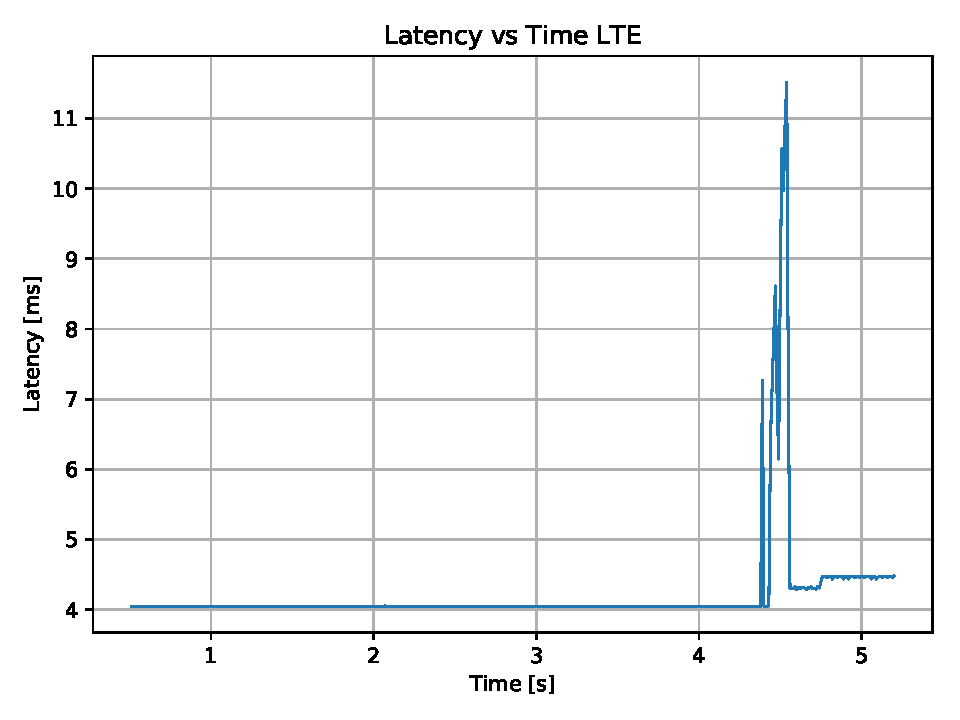
\includegraphics[scale=0.28]{latency_lte_UDP}
				\end{figure}
				\begin{figure}
					\vspace{-0.2in}
					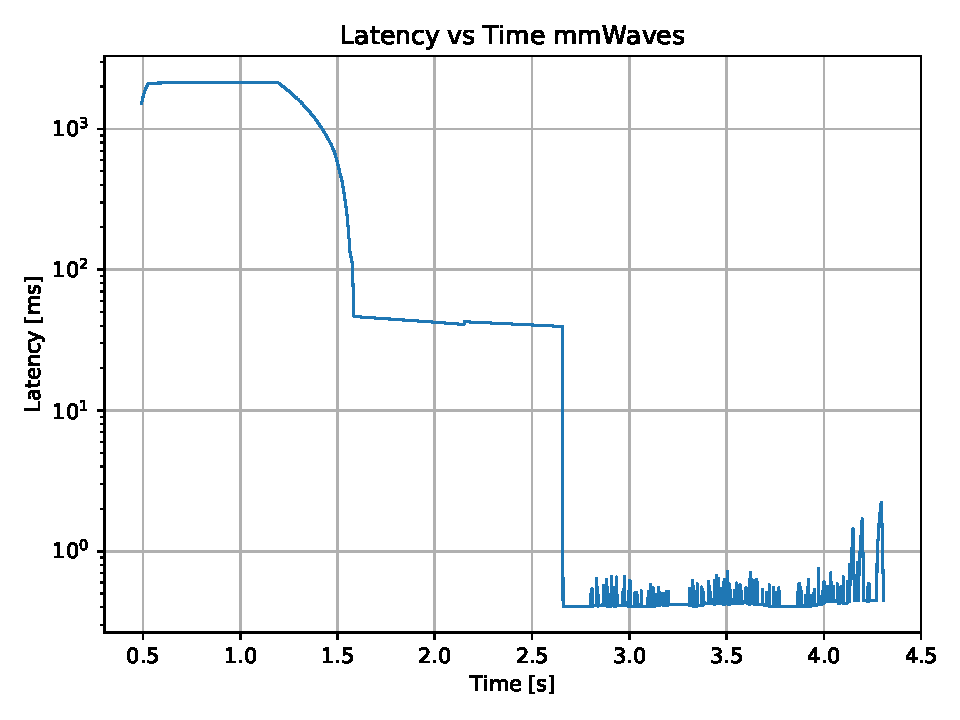
\includegraphics[scale=0.28]{latency_mmWaves_UDP}
				\end{figure}
		\end{columns}
	\end{frame}

	\section{Conclusions}
	\begin{frame}{Conclusions}
		\textbf{DSRC}
		\begin{itemize}
			\item Uses standard IEEE 802.11 frequency band (5.9GHz), suitable for a dense urban enviornment
			\item Lower datarate implies slower communications
		\end{itemize}
		\textbf{LTE}
		\begin{itemize}
			\item Low frequency but higher datarate, suitable for faster communications in dense urban enviroment
			\item Can not reach mmWave's datarates
		\end{itemize}
		\textbf{mmWaves}
		\begin{itemize}
			\item Very high frequency implies very high datarates
			\item High sensitivity to blockages (buildings, people, environment conditions)
		\end{itemize}
	\end{frame}
\end{document}
